\chapter{Introducción específica} % Main chapter title

\label{Chapter2}

%----------------------------------------------------------------------------------------
%	SECTION 1
%----------------------------------------------------------------------------------------
%
%En este capítulo deberías tener:
%1. Conversores AD.  Describir con detalles técnico lo básico de la tecnología que usaste, con lo necesario para que se comprenda lo que sigue en el cap 3.  Usar citas bibliográficas.  Explicar el proceso de cuantización, codificación, el error en la conversión, bits de resolución, ruido, etc.
%Acá podría ir cualquier otro aspecto tecnológico/herramientas que hayas utilizado y quieras documentar, por ejemplo protocolos de comunicación o aspectos metodológicos que hayas seguido como TDD o uso de repositorios de software, etc.
%2. Planificación. Aspectos relevantes de la planificación que ayuden a entender cómo se hizo el trabajo.  El AoN suele ser adecuado para eso.  Algo que te sirva para retomarlo en las conclusiones (riesgos,supuestos,gantt,etc)
%3. Requerimientos
%

%Explicar los detalles que el lector debe conocer para entender las decisiones de diseño adoptadas.
A continuación se describirán diferentes tecnologías usadas en el trabajo que hicieron posible al trabajo desarrollado.

\section{Microcontrolador principal}
\label{sec:cap2parte1}

El trabajo realizado implicó el desarrollo de un producto electrónico que debe realizar diferentes tareas, como medir comunicar y en algunos casos accionar, uno de los elementos que hace posible el funcionamiento del sistema es el microcontrolador, que es el encargado de realizar las diferentes tareas que el dispositivo debe llevar a cabo. En este sistema embebido el microcontrolador ocupa un rol principal pues las demás estructuras que se diseñan dependen de este para funcionar, o mejor dicho se diseñan para ser controladas por este. Para este trabajo se opto por un microcontrolador que pueda ser usado para una aplicación de medición, siendo una de sus propiedades ser de bajo consumo eléctrico. 

%Como toda aplicación de un sistema embebido, la electrónica diseñada suele ser mas una extension del microcontrolador, adaptado analógicamente para que realice las tareas que se desea resolver, que una parte más de la electrónica.

El microcontrolador elegido para el dispositivo fue un MSP430F2618 fabricado por la empresa Texas Instrument, este microcontrolador es de ultra baja potencia con una CPU de instrucciones RISC de 16 bits. Posee periféricos analógicos y digitales orientado a aplicaciones de medición. Este microcontrolador puede pasar de varios modos de baja potencia a modo activo en menos de 1 microsegundo, este puede observarse en la figura\ref{fig:msp430imagen}.

\begin{figure}[!h]
	\centering
	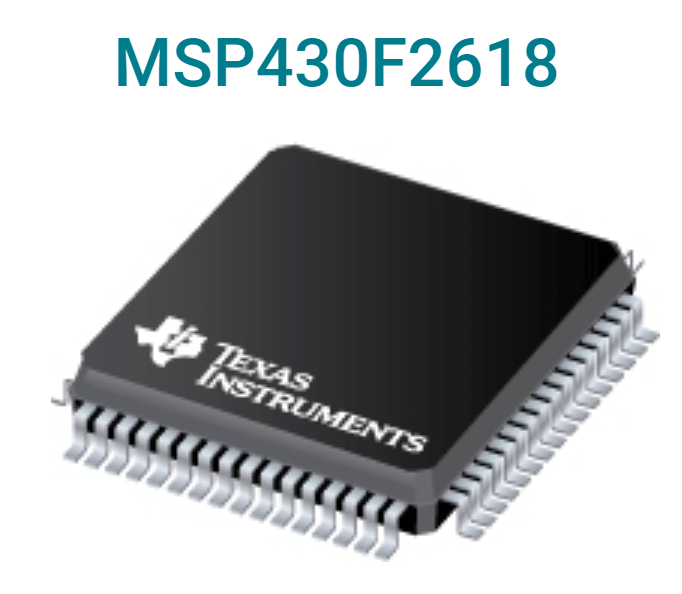
\includegraphics[width=40mm,keepaspectratio]{Figures/msp430F2618.png}
	\caption{Ilustración del micro controlador como se lo presenta en la pagina web del fabricante.}
	\label{fig:msp430imagen}
\end{figure}

El msp430F2618 pose varios tipos de periféricos ideados para diferentes aplicaciones, a cada uno de estos el fabricante los denomina como "módulos". Estos módulos son soluciones de hardware fáciles de implementar por lo que hacen al código mas sencillo. 

Este modelo de la familia msp430 se eligió específicamente por poseer tanto un modulo ADC (conversor analógico - digital) como un modulo DAC (conversor digital-analógico). El modulo DAC fue utilizado para la implementación de un lazo de corriente, que es una forma de comunicación común para procesos industriales. Por otra parte, el modulo  ADC se planteo en un primer momento para las mediciones, su uso fue descartado.  

Para el trabajo se uso el modulo de comunicación serie universal para realizar la comunicación con el integrado de medición como también para realizar los protocolos de comunicación requeridos. El microcontrolador posee un oscilador interno por lo que no necesita de uno externo para funcionar, sin embargo se decidió usar un oscilador externo para asegurar la estabilidad de las comunicaciones seriales como también para aumentar la precisión de los módulos temporizadores que se implementaron.

\begin{figure}[!h]
	\centering
	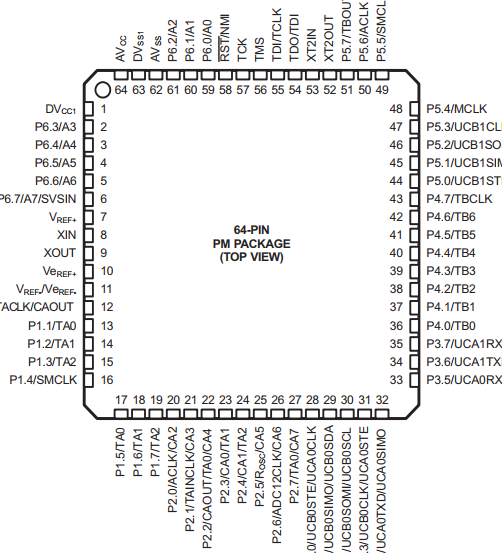
\includegraphics[width=60mm,keepaspectratio]{Figures/microdatasheet1.png}
	\caption{Esquemático del micro controlador.}
	\label{fig:msp430squematic}
\end{figure}

En cuanto al empaquetado del dispositivo se opto por el de 64 pines de salida (denominado por el fabricante como "LQFP-64 Texas Instruments" este puede verse en la figura \ref{fig:paquet64}., esta version a diferencia del empaquetado de 80 pines posee mas de una implementación de módulos por pin, debido a que no se iban a usar todas las prestaciones del microcontrolador esto no presentaba un problema. 

\begin{figure}[!h]
	\centering
	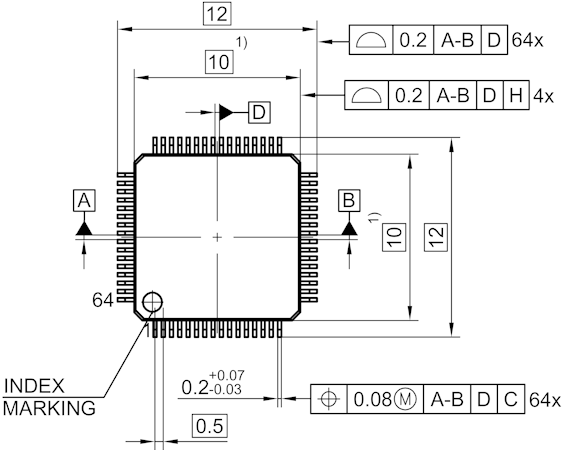
\includegraphics[width=80mm,keepaspectratio]{Figures/PG-LQFP-64-18.png}
	\caption{Dimensiones del empaquetado LQFP-64 (valores en milímetro).}
	\label{fig:paquet64}
\end{figure}

El empaquetado de montaje superficial es de un tamaño bastante pequeño (sus dimensiones son de 12x12mm) por lo que presentaba un pequeño desafío al implementarlo en el diseño del PCB.


\section{Herramientas de programación}
\label{sec:cap2parte2}
\subsection{FET debugger}

Para lograr que el microcontrolador realice todas las tareas requeridas se debe programarlo para tal fin, es decir se debe escribir las instrucciones que deberá seguir el microcontrolador. El conjunto de instrucciones que se escriben para que un microcontrolador funcione es a lo que denominamos programa, y en este trabajo se llamara firmware. El firmware debe cargarse de algún modo desde la computadora personal donde lo diseñamos al chip. 

Para cargar el programa al microcontrolador, el fabricante especifica una herramienta de programación, a esta herramienta lo denomina  "FET hardware JTAG",puede verse en la figura \ref{fig:mspFETtool}, siendo FET acrónimo de "Flash Emulation Tool" y JTAG acrónimo de Joint Test Action Group. El JTAG es un estándar industrial para verificar diseños y testear placas de circuito impresas después de manufacturadas \cite{JTAGintel}. Los programadores JTAG son usados para escribir software en memorias flashes.
%citar el resumen de intel del ieee

\begin{figure}[!h]
	\centering
	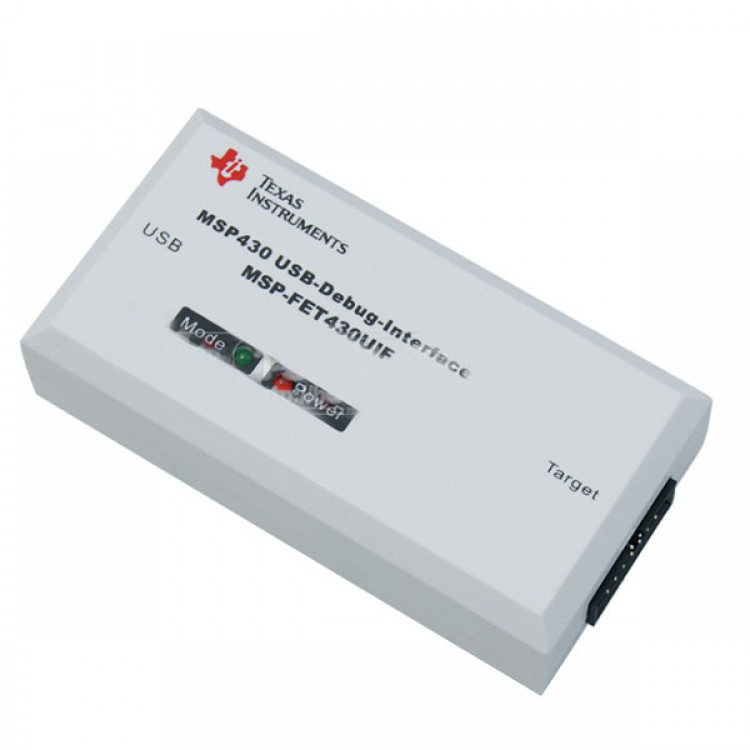
\includegraphics[width=100mm,keepaspectratio]{Figures/emeesepeFET.jpg}
	\caption{ Foto del MSP-FET430UIF, que es la herramienta de programación del microcontrolador.}
	\label{fig:mspFETtool}
\end{figure}

Con las conexiones apropiadas un debugger y la interfaz JTAG pueden ser usadas para \textit{debuggear} código en el microcontrolador, esto facilita la programación de prototipos a realizar. El cable utilizado para conectar la herramienta a través de una interfaz JTAG puede verse en la figura \ref{fig:mspFETtool}, esta interfaz daba una idea de como debía ser la conexión en la placa electrónica del prototipo.

%The typical MSP Flasher execution flow consists of the following steps. Optional steps can be activated or
%deactivated by using special triggers or parameters (see Section 3).
%1. Initialize FET debugger
%2. Perform FET recovery (if a corrupted FET firmware is detected)
%3. Update FET firmware (if a mismatch between firmware and MSP Debug Stack versions is detected)
%4. Power up the target MSP device
%5. Configure the target MSP for JTAG or SBW communication
%6. Connect to the target MSP and display device information
%7. Optional: Erase (parts of) the target device memory
%8. Optional: Load target code into the device from a TXT or HEX file
%9. Optional: Verify target code transfer
%10. Optional: Read device memory and write it to a TXT or HEX file
%11. Optional: Reset the device
%12. Optional: Lock JTAG access
%13. Optional: Reset the device
%14. Optional: Power down the device
%15. Optional: Start target code execution
%16. Disconnect from the target MSP device
%17. Close the FET connection

%citar datasheet del msp

\begin{figure}[!h]
	\centering
	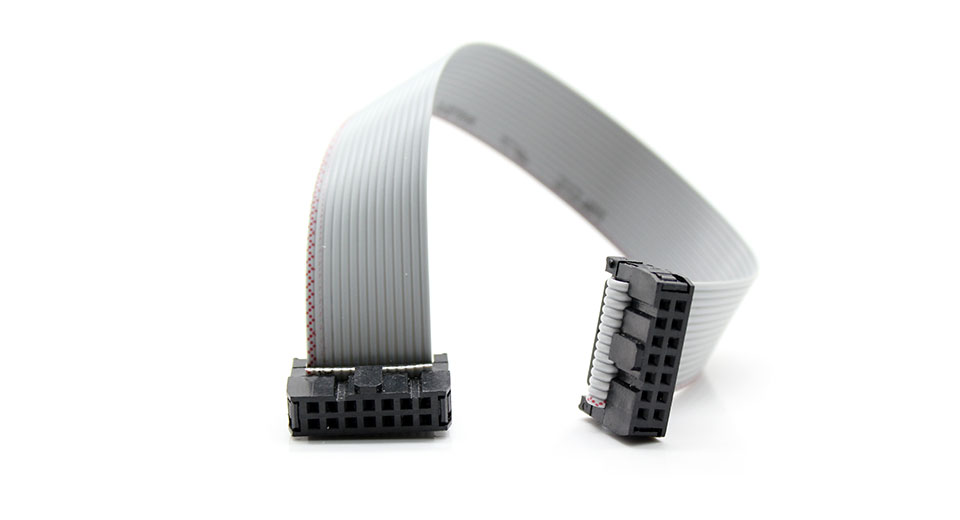
\includegraphics[width=120mm,keepaspectratio]{Figures/cableJtag.jpg}
	\caption{ Cable conector de la interfaz JTAG. }
	\label{fig:mspFETtool}
\end{figure}

En la hoja de datos de la herramienta, el fabricante especifica las conexiones y funciones de cada pin, esto fue tomado en cuenta para el diseño del esquemático del prototipo, en el cual se optó por una interfaz JTAG Through-Hole, esto se detallara en el siguiente capitulo. 

\begin{figure}[!h]
	\centering
	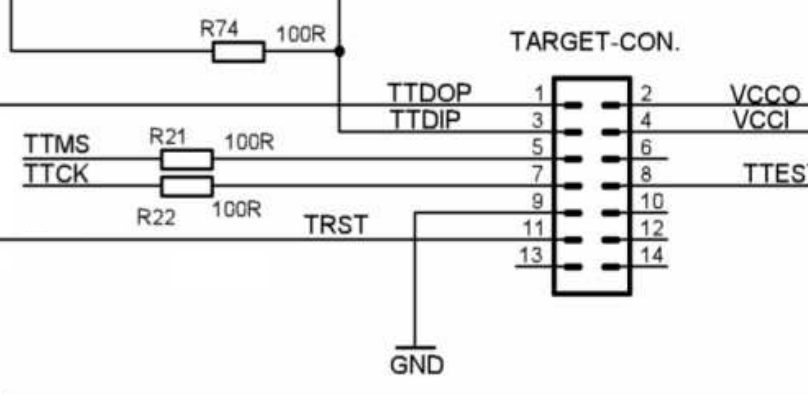
\includegraphics[width=100mm,keepaspectratio]{Figures/Jtagfetsch.png}
	\caption{ Esquemático del conector JTAG de la herramienta de programación.. }
	\label{fig:FETtoolsch}
\end{figure}

%The MSP debug stack (MSPDS) for all MSP430™ microcontrollers (MCUs) and SimpleLink™ MSP432™ devices consists of a static library on the host system side as well as an embedded firmware that runs on debug tools including the MSP-FET, MSP-FET430UIF or on-board eZ debuggers. It is the bridging element between all PC software and all MSP430 and SimpleLink MSP432 microcontroller derivatives and handles tasks such as code download, stepping through code or break points. The MSP Debug Stack is used in integrated development environments such as Code Composer Studio™ (CCS), IAR's Embedded Workbench or tools like Smart RF Studio and Elprotronic's FlashPro430.


\subsection{Entorno de desarrollo}

Para poder programar el microcontrolador el fabricante ofrece una solución de software denominado "MSPDS" que significa MSP Debug stack. El MSPDebug stack es una librería dinámica que provee funciones para controlar y debuguear el



El "stack debug de MSP" es diseñado para los microcontroladores de la familia MSP430, consiste en una librería estática en el lado del host (donde se realizan los programas) y de un firmware embebido que corre herramientas de debugging para el MSP-FET.\cite{GuideMSPStack}

\begin{figure}[h]
	\centering
	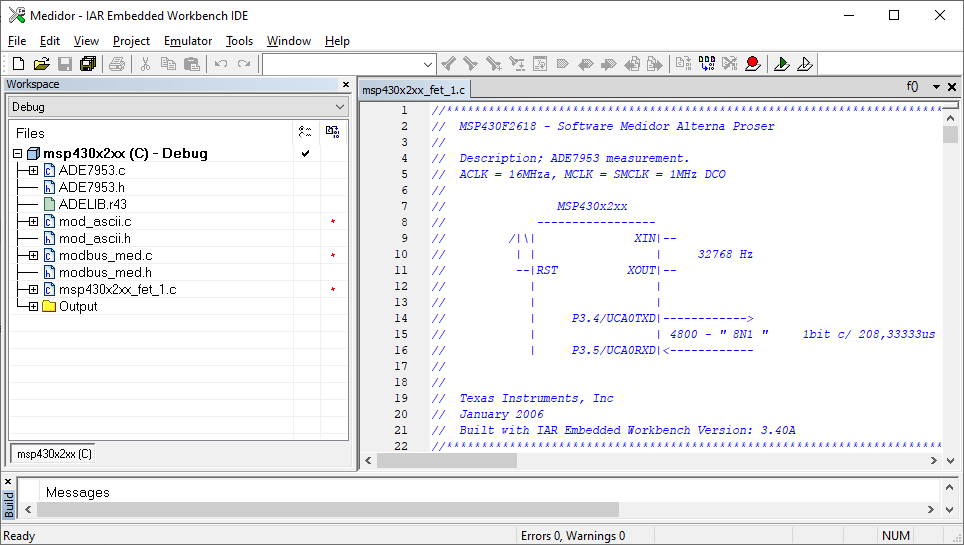
\includegraphics[width=110mm,keepaspectratio]{Figures/Embeddedworkbench.png}
	\caption{Imagen del entorno de desarrollo.}
	\label{fig:IARwindow}
\end{figure}

%citar datashet del fet

\section{Circuito integrado de medición}
\label{sec:cap2parte3}

JTAG (named after the Joint Test Action Group which codified it) is an industry standard for verifying designs and testing printed circuit boards after manufacture.
Although JTAG's early applications targeted board level testing, here the JTAG standard was designed to assist with device, board, and system testing, diagnosis, and fault isolation. Today JTAG is used as the primary means of accessing sub-blocks of integrated circuits, making it an essential mechanism for debugging embedded systems which 

%
%
With the proper connections, the debugger and an FET hardware JTAG interface (such as the
MSP-FET430PIF and MSP-FET430UIF) can be used to program and debug code on the target board. In
addition, the connections also support the MSP-GANG430 or MSP-PRGS430 production programmers,
thus providing an easy way to program prototype boards, if desired.

JTAG programmers are also used to write software and data into flash memory. This is usually done using the same data bus access the CPU would use, and is sometimes handled by the CPU. In other cases the memory chips themselves have JTAG interfaces. Some modern debug architectures provide internal and external bus master access without needing to halt and take over a CPU. In the worst case, it is usually possible to drive external bus signals using the boundary scan facility.

This manual describes the hardware of the Texas Instruments MSP-FET430 Flash Emulation Tool (FET).
The FET is the program development tool for the MSP430 ultra-low-power microcontroller. Both available
interface types, the parallel port interface and the USB interface, are described.


If you intend to program your MSP430 or MSP432 device out of an IDE, simply download the latest version of Code Composer Studio or IAR Embedded Workbench release. The latest MSP Debug Stack will be included.

Para realizar el programa en lenguaje c y descargarlo en el microcontrolador la empresa SERVAIND S.A. proveyó un entorno de desarrollo privado y una placa electrónica con el microcontrolador funcionando, de modo de probarla. Una ventana del entorno de desarrollo puede verse en la figura \ref{fig:IARwindow}.


%\subsection{Uso de mayúscula inicial para los título de secciones}

\section{ Libreria Externa - Free Modbus}
\label{sec:cap2parte3}
%https://github.com/cwalter-at/freemodbus


%cite https://www.ti.com/tool/MSPDS#descriptionArea


%\protect\footnotemark[1]
%\footnotetext[1]{\url{https://goo.gl/images/i7C70w}}
